The following section aims to provide an in-depth overview of the system's architecture as well as the rationale for major design decisions taken during the implementation.

\subsection{System architecture and execution control flow}
% todo overview, add class diagrams and flow charts

\subsection{Instruction translation process}
% todo

\subsection{Code cache and TLB for block lookup}
% todo

\subsection{Static hybrid register mapping}
\subsubsection{Register priority analysis}
In order to achieve the best performance with the hybrid approach to the register mapping described in section \vref{sec:context-switch-reg-handle}, we must decide which registers of the RISC-V guest to map into the host's limited number of available GPRs.
There are two main ways of determining the priority of registers when considering them as candidates for a mapping.

It is, on the one hand, possible to assess the priority statically, by performing an analysis of the binary in question.
Essentially, the hereby produced metric counts the number of times the register is used in the assembly instructions listed in the guest program and thus delivers an idea of how important each register is to this specific executable.
We have built the tools required for this effort directly into the translator's analyser function, accessed via the \texttt{-a} flag (see appendix \ref{sec:appendix-tools}).

However, this approach does not take into account that a single instruction may be executed many times while the program is running.
Accordingly, the other approach is to assess the register priority dynamically by analysing and profiling the execution of the testing program, thereby gaining an insight into how often each register is actually used during the execution.
The translator is also capable of performing such an analysis, commanded by the \texttt{-p} flag.
A dynamic analysis, of course, delivers a largely more accurate idea of the priority of the registers in question, but has the decided and obvious disadvantage that it cannot be performed without actually executing the binary.

\begin{table}
	\centering
	\makebox[\textwidth][c]{%
		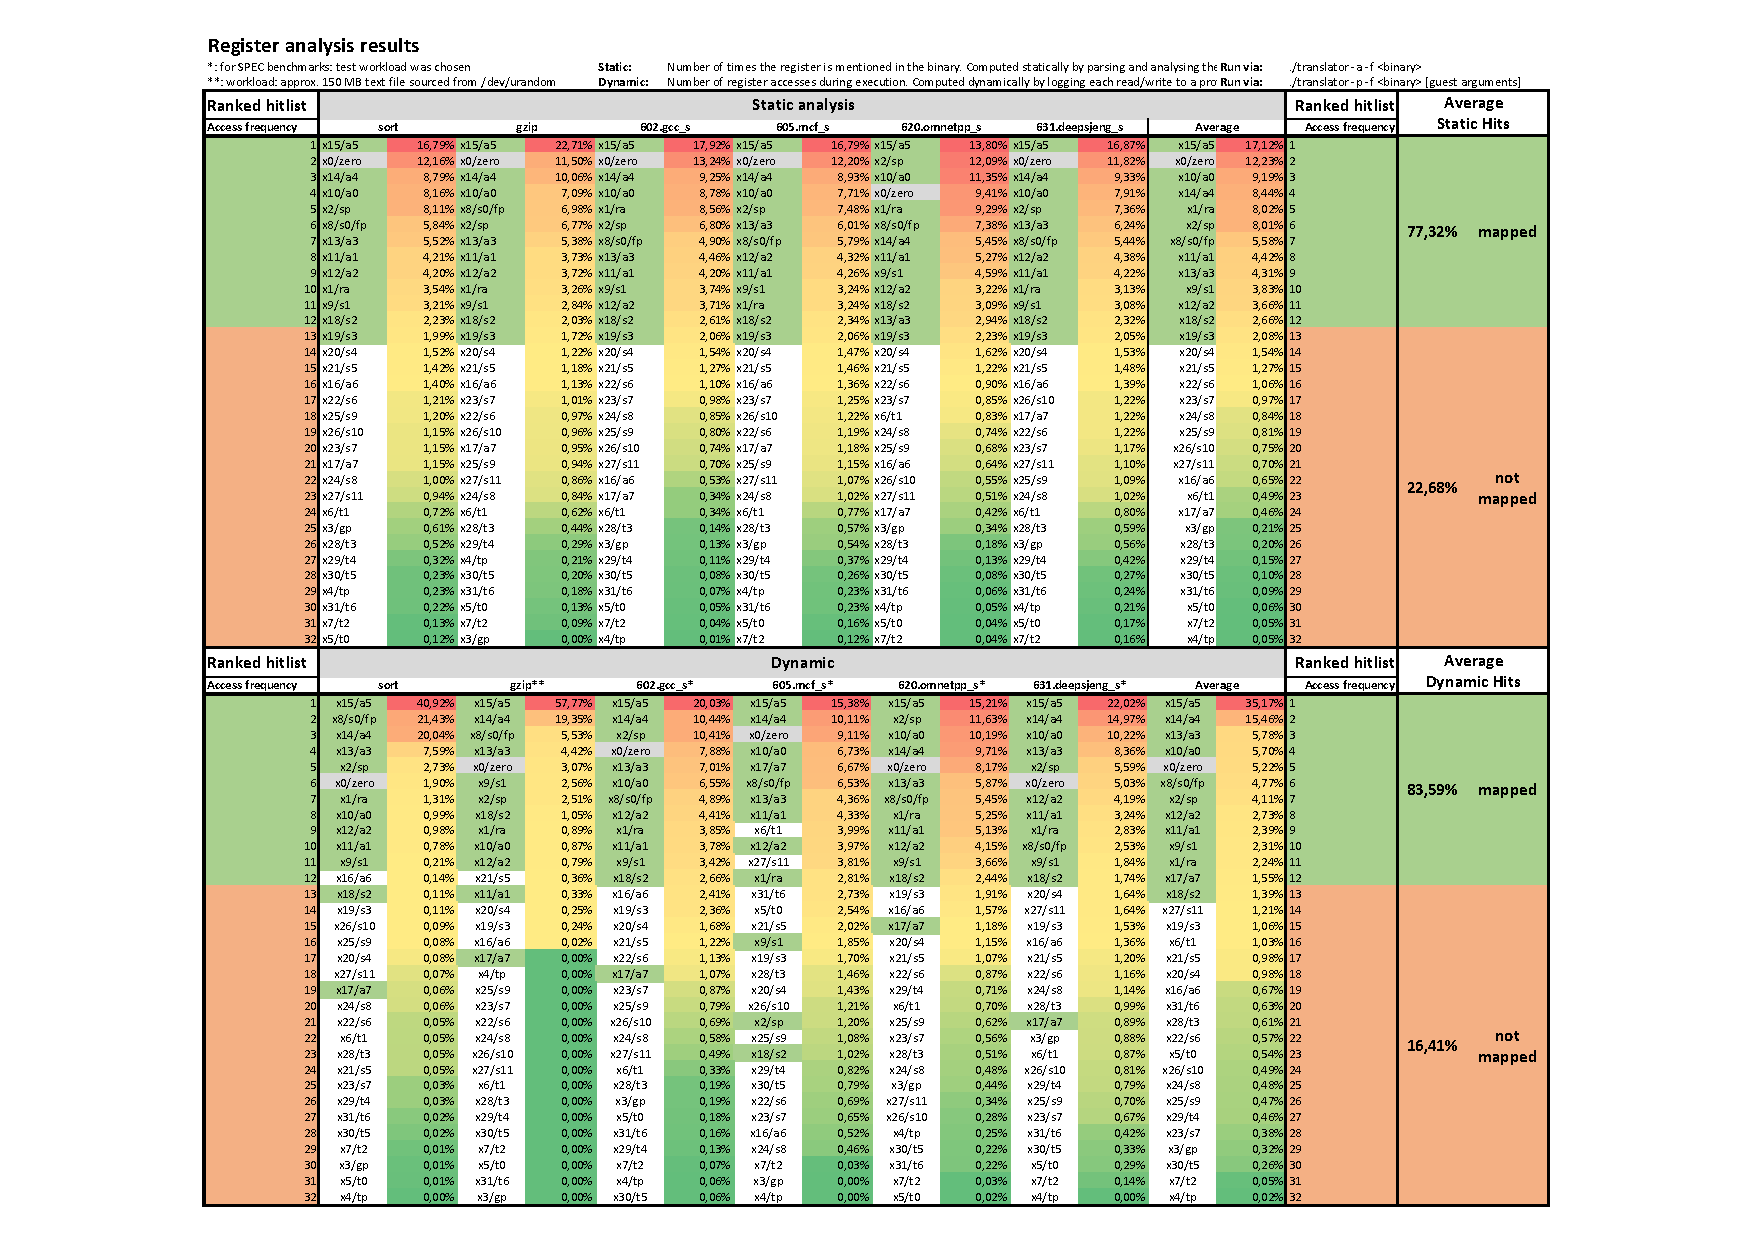
\includegraphics[height=1.17\textwidth,angle=90]{media/register-usage}%
	}
	\caption{The results of a static and dynamic register usage analysis of several \textit{SPEC CPU 2017} benchmarks, \textit{gzip} as well as a merge sort utility program.}
	\label{tab:register-analysis-results}
\end{table}

For the results of such an analysis performed on a range of programs, including \textit{gzip}~\cite{gzip} and several benchmarks of the \texttt{intspeed}-Suite of \textit{SPEC CPU 2017}~\cite{spec-cpu-2017}, see table \vref{tab:register-analysis-results}.
Primarily, we gain interesting insights into the differences between the static and dynamic results yielded by the analysis.
While the static ranked hit list does not differ greatly between the different executables and the top $12$ entries are identical for every one of the tested programs, the dynamic results are far more variable.
This makes creating a register mapping that fits well to every executable very difficult.

The benchmarks \texttt{605.mcf\_s} (route planning workload) and \texttt{620.omnetpp\_s} (discrete event simulation for computer networking)~\cite{spec-cpu-doc} of the \textit{SPEC CPU} suite can serve as examples here.
For programs like \texttt{605.mcf\_s} that only lightly use the stack, holding the stack pointer \texttt{sp/x2} in a native register when only $1,20\,\%$ of accesses actually utilise it would not be necessary.
However, other programs like \texttt{620.omnetpp\_s} may rely heavily on the stack, and thus log very frequent accesses to \texttt{sp/x2};
when statistically every ninth access is to the stack pointer, it is absolutely essential to map the register to a native GPR.

If a static analysis yielded results of similar quality to the dynamic counterpart, the DBT could analyse the binary prior to execution and run every program with a best-fit static register mapping.
However, evidently, this is impossible with dynamic profiling.


\subsubsection{Structure of the mapping}
When we structure our mapping by the average case of the insights gained, we statistically capture about $83,59\,\%$ of register accesses, leaving the remaining $16,41\,\%$ to read from the register file in memory.

From the 16 general-purpose registers x86-64 has to offer, we may use the 12 registers \texttt{rbx}, \texttt{rbp}, \texttt{rsi}, \texttt{rdi} and \texttt{r8}--\texttt{r15}.
The remaining registers have either implicit or exclusive functions in some instructions (\texttt{rax} and \texttt{rdx} for multiplication/division, \texttt{cl} for shifting), or, like \texttt{rsp}, are impractical to use in combination with block chaining and function calls.

Taking the 12 registers that are most accessed on average, the mapping structure is as seen in table \vref{tab:static-register-mapping}.

\begin{table}
	\centering
	\begin{tabular}{rcccccccccccc}
		\toprule
		\textbf{RISC-V register} & \texttt{a5} & \texttt{a4} & \texttt{a3} & \texttt{a0} & \texttt{fp} & \texttt{sp} & \texttt{a2} & \texttt{a1} & \texttt{s1} & \texttt{ra} & \texttt{a7} & \texttt{s2}\\
		\textbf{x86-64 mapping} & \texttt{rbx} & \texttt{rbp} & \texttt{rsi} & \texttt{rdi} & \texttt{r8} & \texttt{r9} & \texttt{r10} & \texttt{r11} & \texttt{r12} & \texttt{r13} & \texttt{r14} & \texttt{r15}\\
		\bottomrule
	\end{tabular}
	\caption{The static register mapping in use by the translator.}
	\label{tab:static-register-mapping}
\end{table}

\subsubsection{Register file memory access}
Continued here\ldots
% todo about register loads in instructions


\subsection{Context switching details}
% todo context switching

\subsection{Optimisation of the generated code}
\subsubsection{Block chaining}
\subsubsection{Recursive jump translation}
\subsubsection{Macro operation fusion}
% todo optimisation details, maybe split up? more sections?

\subsection{Detailed system call overview}
% todo special description for emulated calls

As described in section \vref{sec:syscall-handling}, we must assume the role of the kernel by handling system calls during the execution of the guest program.
We achieve this by translating the \texttt{ECALL} instruction as a context switch and jump to the \texttt{emulate\_ecall} routine in the DBT, which can then take the appropriate action.

As we stored the guest's registers before jumping to the handler, the requested system call index is now available to the DBT in the register file as entry \texttt{a7}, as per the RISC-V standard calling convention.
We may now handle the system calls based on that index and the arguments passed in the registers \texttt{a0} through \texttt{a6}, and write the return value to entry \texttt{a0} of the register file prior to switching the context back to the guest.

As previously mentioned, some system calls require special handling when encountered by the DBT (see table \vref{tab:syscall-special} for details).
The following will describe the specifics of these issues with system calls that are either not present on the x86-64 host architecture, or may influence or break the state of the DBT.
\begin{description}
	\item[Adapting structure data format.]
	There are system calls like \texttt{fstat} and \texttt{fstatat} that exist both on RISC-V as well as x86-64, but use different data structure layouts in their return values.
	Thus, the DBT must adapt the host's returned data to the required format prior to passing it back to the guest.
	
	
	\item[Emulation required.]
	The DBT captures the \texttt{exit} and \texttt{exit\_group} calls.
	Passing them through would immediately terminate the DBT -- an action that is undesirable as it prevents any form of clean-up or post-execution profiling and analysis to take place.
	Thus, the DBT uses these system calls to set a flag which stops the translator's main loop from executing the next iteration.
	
	The \texttt{brk} system call must also be entirely emulated, as it would otherwise allow the guest program to modify the endpoint of the DBT's data segment (\textit{program break}), thus potentially deallocating some of the translator's memory.
	
	
	\item[Ignoring system calls.]
	% todo expand the rationale here. is this correct?
	The \texttt{rt\_sigaction} system call is ignored by the DBT, as any signals received by the process will be handled by the translator due to the fact that the guest program's execution is emulated in the DBT's process.
	
	
	\item[Guarded pass-through to host.]
	Essentially, any system call that has the possibility to influence the state or memory of the translator needs to have respective safe-guards in place.
	A good example of this behaviour is the \texttt{mmap} system call, the handling of which also reflects the memory layout scheme discussed in section \vref{sec:memory-layout}.
	
	In any case, we must prevent a memory mapping into the translator's memory region.
	Mappings that do not interfere with the DBT's memory can be passed along to the host directly.
	In case a hinted mapping would conflict with the translator's memory, we may just re-hint the mapping to the top of the guest's address space.
	When the call is not hinted (the \texttt{MAP\_FIXED} or \texttt{MAP\_FIXED\_NOREPLACE} flag commands the mapping at exactly the specified address), we are unable to provide the guest with the requested mapping; thus we simulate an existing mapping in the location in question by returning \texttt{EEXIST} for \texttt{MAP\_FIXED\_NOREPLACE} and failing the call with \texttt{EINVAL} for \texttt{MAP\_FIXED}.
	
	Similarly, we fail the guest's \texttt{munmap} with \texttt{EINVAL} in cases where the translator's memory would be compromised by the deallocation.
\end{description}

The other supported system calls may be directly passed through to the host after performing the necessary index mapping (see table \vref{tab:syscall-pass-through}).

\begin{table}
	\centering
	\begin{tabular}{ccc}
		\toprule
		\textbf{System Call (index)} & \textbf{Handling} & \textbf{x86-64 base (index)}\\ 
		\midrule
		\texttt{fstatat} (79) & data reformat & \texttt{newfstatat} (262)\\
		\texttt{fstat} (80) & data reformat & \texttt{fstat} (5)\\
		\texttt{exit} (93) & emulate & n/a\\
		\texttt{exit\_group} (94) & emulate & n/a\\
		\texttt{rt\_sigaction} (134) & ignore & n/a\\
		\texttt{brk} (214) & emulate & n/a\\
		\texttt{munmap} (215) & guarded pass-through & \texttt{munmap} (11)\\
		\texttt{mmap} (222) & guarded pass-through & \texttt{mmap} (9)\\
		\bottomrule
	\end{tabular}
	% todo keep up-to-date
	% state: aa55cef4816eb790df21f4742b7cf1f29685da49
	\caption{An overview of the system calls we support that require special handling by the binary translator.}
	\label{tab:syscall-special}
\end{table}

\begin{table}
	\centering
	\begin{tabular}{rlc}
		\toprule
		\textbf{RISC-V system call} & \textbf{\ldots index} & \textbf{x86-64 index}\\
		\midrule
		\texttt{getcwd} & 17 & \refer 79\\
		\texttt{fcntl} & 25 & \refer 72\\
		\texttt{ioctl} & 29 & \refer 16\\
		\texttt{unlinkat} & 35 & \refer 263\\
		\texttt{faccessat} & 48 & \refer 269\\
		\texttt{chdir} & 49 & \refer 80\\
		\texttt{fchmod} & 52 & \refer 91\\
		\texttt{fchown} & 55 & \refer 93\\
		\texttt{pipe2} & 59 & \refer 293\\
		\texttt{openat} & 56 & \refer 257\\
		\texttt{close} & 57 & \refer 3\\
		\texttt{getdents64} & 61 & \refer 217\\
		\texttt{lseek} & 62 & \refer 8\\
		\texttt{read} & 63 & \refer 0\\
		\texttt{write} & 64 & \refer 1\\
		\texttt{writev} & 66 & \refer 20\\
		\texttt{readlinkat} & 78 & \refer 267\\
		\texttt{utimensat} & 88 & \refer 280\\
		\texttt{set\_tid\_address} & 96 & \refer 218\\
		\texttt{futex} & 98 & \refer 202\\
		\texttt{set\_robust\_list} & 99 & \refer 273\\
		\texttt{clock\_gettime} & 113 & \refer 228\\
		\texttt{tgkill} & 131 & \refer 234\\
		\texttt{rt\_sigprocmask} & 135 & \refer 14\\
		\texttt{uname} & 160 & \refer 63\\
		\texttt{gettimeofday} & 169 & \refer 96\\
		\texttt{getpid} & 172 & \refer 39\\
		\texttt{getuid} & 174 & \refer 102\\
		\texttt{geteuid} & 175 & \refer 107\\
		\texttt{getgid} & 176 & \refer 104\\
		\texttt{getegid} & 177 & \refer 108\\
		\texttt{gettid} & 178 & \refer 186\\
		\texttt{sysinfo} & 179 & \refer 99\\
		\texttt{execve} & 221 & \refer 59\\
		\texttt{wait4} & 260 & \refer 61\\
		\texttt{prlimit64} & 261 & \refer 302\\
		\texttt{renameat2} & 276 & \refer 316\\
		\texttt{getrandom} & 278 & \refer 318\\
		\bottomrule
	\end{tabular}
	% todo keep up-to-date
	% state: aa55cef4816eb790df21f4742b7cf1f29685da49
	\caption{An overview of the system calls handled via pass-through to the host.}
	\label{tab:syscall-pass-through}
\end{table}








